\section{Calibration}\label{sec:calibration}

The quantitative exercise combines an end-2024 exposure network for Germany (DEU), France (FRA), Italy (ITA) and Spain (ESP) with a sovereign-crisis scenario. The matrix and reported balance sheets determine the positions at risk. Public capital data and the scenario specify when losses trigger costly distress. Appendix~\ref{app:calibration-details} gives the numerical implementation; the Online Appendix documents the source data and reconstruction.

\subsection{The exposure network}

The database combines ECB bank balance sheets and securities holdings, Eurostat financial accounts and International Monetary Fund (IMF) portfolio positions. The choice of a common residence basis is driven by data availability and the need to combine these public sources with consistent institutional coverage. A country's bank block includes banking offices located there, including foreign-owned offices, and excludes offices abroad, including those owned by domestic banking groups. Worldwide consolidated bank data would instead include foreign affiliates whose assets and liabilities fall outside the resident sectors measured by the other sources.

Within this residence-based network, we use public ECB information to estimate and remove loans between offices of the same banking group. We retain the remaining domestic interbank claims without netting them against matching liabilities: each national bank block represents distinct institutions sharing a repayment rate.\footnote{The ECB data report aggregate loan and deposit positions between offices of the same group, rather than a complete bilateral matrix. The Online Appendix explains how we allocate these amounts and remove the corresponding loans where the available data permit. Positions without a public breakdown are not assumed absent. This adjustment does not amount to worldwide group consolidation.} This choice matters for repayment feedback. In an alternative calculation, netting domestic interbank assets against the corresponding liabilities eliminates multiplicity at the reference parameters (Appendix~\ref{app:ocr_robustness}).

The public sources provide totals by instrument and some counterparty detail, but no complete bilateral exposure matrix. We reconstruct missing positions using the available totals and counterparty information, and reconcile discrepancies across sources as documented in the Online Appendix. The results are conditional on this reconstruction.

Sovereign bond holdings are reconciled to official debt-security totals, and household claims on banks comprise deposits and securities holdings. The exposure matrix covers selected instruments; we reconcile it with complete bank balance sheets to obtain repayment resources and clearing debts while retaining full accounting equity. Obligations settled outside the common repayment pool are deducted from both resources and debt.

Figure~\ref{fig:calibrated-exposure-network} isolates the sovereign and interbank exposures at the centre of the spillover mechanism. Arrow widths measure each claim relative to the creditor banking system's reported total assets. Table~\ref{tab:bank-exposures} reports the same positions in amounts and as percentages of total assets, with one column per creditor banking system. Italian and Spanish banks' domestic sovereign holdings stand out, while domestic interbank claims are particularly large in Germany and France. The loops represent claims between distinct banks within a national block. Sovereigns are passive nodes: their repayments depend on the sovereign state, whereas banks' repayments respond to their counterparties. Appendix~\ref{app:calibration-details}, Figure~\ref{fig:full-exposure-network}, shows the broader sector network.

\begin{figure}[t]
\centering
\floatcaption{Bank exposures to sovereigns and banking systems, end-2024}{Arrows run from creditor banks to debtor banks or sovereigns; their widths are proportional to the claim divided by the creditor banking system's reported total assets. All 32 bank--bank and bank--sovereign positions are represented, including very small foreign exposures. Colours identify the creditor's country, as in Figure~\ref{fig:full-exposure-network}. Labels give domestic exposures as percentages of total assets. Loops are domestic claims between distinct institutions after the related-office adjustment. Sovereigns have no outgoing arrows. Other asset classes are omitted from this view; calculations retain the full exposure network.}
\label{fig:calibrated-exposure-network}

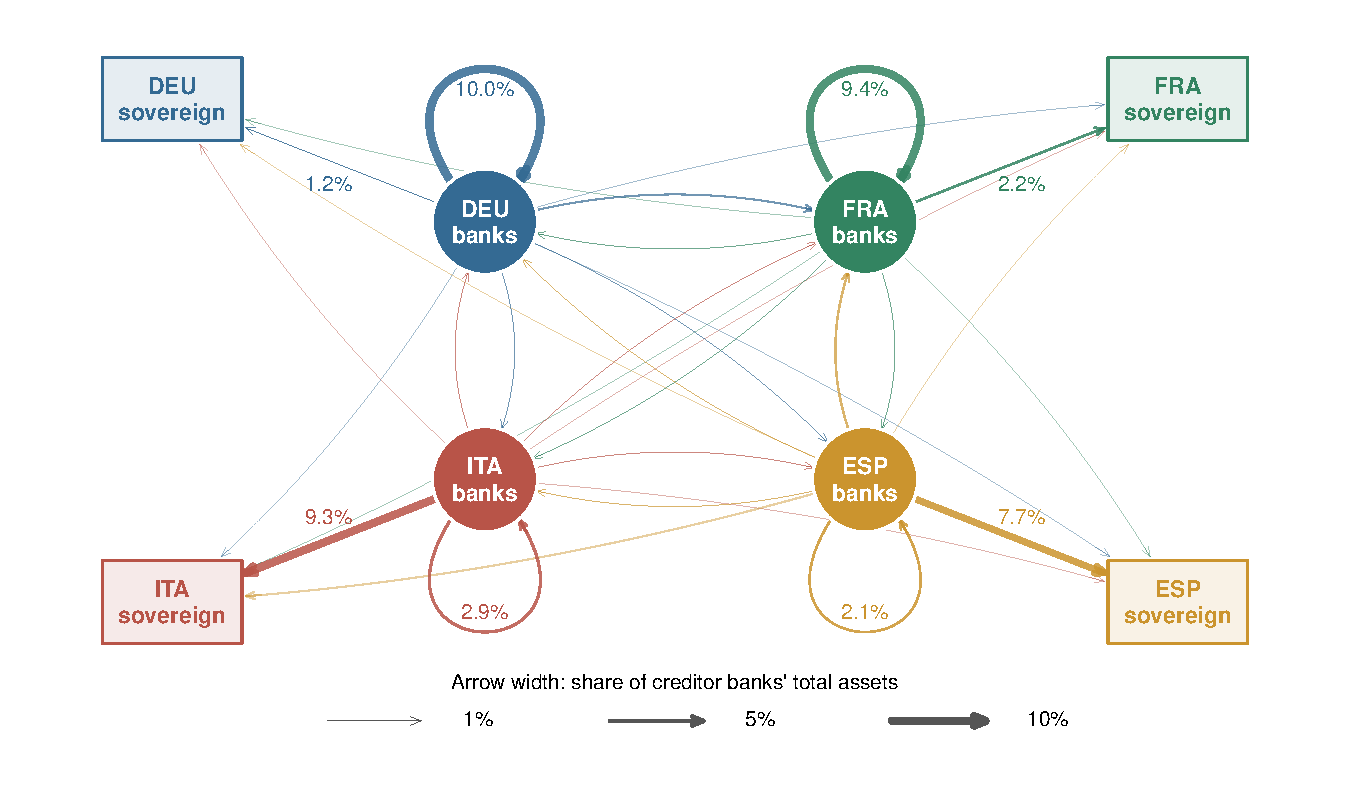
\includegraphics[width=\textwidth]{Figures/bank_exposure_network.pdf}

\end{figure}

\begin{table}[htbp]
\centering
\floatcaption{Bank exposures to sovereigns and banking systems, end-2024}{Columns identify creditor banking systems; rows identify debtor sovereigns or banking systems. Each cell reports EUR billions, followed in parentheses by the percentage of the creditor banking system's reported total assets. The last row gives that denominator in EUR billions. A positive share that rounds to zero at one decimal place is shown as $<0.1\%$. Sovereign exposures are bond holdings; interbank claims include loans and securities after the related-office adjustment. Domestic interbank claims are between distinct institutions. These are the positions shown in Figure~\ref{fig:calibrated-exposure-network}; other assets are outside this table.}
\label{tab:bank-exposures}
\small
\begin{tabular*}{\textwidth}{@{\extracolsep{\fill}}lrrrr@{}}
\toprule
 & Germany & France & Italy & Spain \\
\midrule
\multicolumn{5}{@{}l}{\textit{Sovereign bonds}} \\
Germany & 134.4 (1.2\%) & 0.4 ($<0.1$\%) & 9.8 (0.3\%) & 1.5 ($<0.1$\%) \\
France & 12.1 (0.1\%) & 259.7 (2.2\%) & 26.5 (0.7\%) & 4.3 (0.1\%) \\
Italy & 14.3 (0.1\%) & 8.1 (0.1\%) & 356.8 (9.3\%) & 44.6 (1.4\%) \\
Spain & 10.6 (0.1\%) & 7.5 (0.1\%) & 42.0 (1.1\%) & 236.6 (7.7\%) \\
\addlinespace
\multicolumn{5}{@{}l}{\textit{Claims on banking systems}} \\
Germany & 1,074.8 (10.0\%) & 98.4 (0.8\%) & 13.3 (0.3\%) & 12.8 (0.4\%) \\
France & 151.6 (1.4\%) & 1,103.9 (9.4\%) & 45.2 (1.2\%) & 57.7 (1.9\%) \\
Italy & 23.4 (0.2\%) & 124.7 (1.1\%) & 112.6 (2.9\%) & 24.8 (0.8\%) \\
Spain & 19.6 (0.2\%) & 83.1 (0.7\%) & 10.9 (0.3\%) & 66.4 (2.1\%) \\
\midrule
Total bank assets & 10,801.2 & 11,715.2 & 3,849.0 & 3,092.4 \\
\bottomrule
\end{tabular*}

\end{table}

\subsection{The crisis specification}\label{subsec:calibration_choices}

We set sovereign recovery at 50\% of contractual bond payments, a rounded benchmark consistent with the order of magnitude observed in historical sovereign defaults. Moody's reports an issuer-weighted average recovery rate of 53\% on defaulted sovereign bonds over 1998--2021 \citep{MoodysSovereign2022}.\footnote{Moody's measures recovery using bond trading prices around default or the closing of a distressed exchange; its value-weighted average is lower, at 40\%. Recoveries vary substantially across episodes: the same report records 24\% and 37\% for Greece's two 2012 defaults. These market-value recovery measures motivate the magnitude of our one-period payment assumption, rather than provide an exact estimate for each sample country.}

To turn sovereign bond holdings into repayment resources, we need both the payment following default and the promised payment in its absence. We calibrate the latter using market prices of sovereign default protection: greater default risk implies a higher promised payment, so that each sovereign bond has the same average payoff as the safe asset under these pricing inputs.\footnote{The inputs are derived from sovereign credit default swap (CDS) premiums, the prices paid for protection against sovereign credit events. They reflect market pricing of risk rather than historical default frequencies. Appendix~\ref{app:calibration-details} gives the data, the conversion into default-risk inputs and the payoff formula.} This provides a common pricing benchmark before comparing the losses caused by different sovereign defaults.

The scenario also includes a deterioration in private credit in the country whose sovereign defaults. Using private-credit impairment proxies from the ECB's 2025 bank stress test \citep{ECBStress2025}, we impose losses of 1.8\% on bank loans to firms resident in that country and 1.7\% on bank loans to resident households, regardless of the lending bank's country. These impairments reduce $a_i(s)$, the nonbank repayment resources introduced in Section~\ref{sec:model_banks}, alongside the loss on sovereign bonds. They therefore lower bank resources before interbank repayment feedback and the bank's own default cost. For example, a French sovereign default reduces a German bank's receipts on loans to French firms and households as well as on French government bonds.\footnote{The private-loan loss rates cover a three-year crisis episode and are applied once at settlement. Linking these impairments to the borrower's sovereign-default state is a scenario assumption, not an estimated causal effect. Appendix~\ref{app:calibration-details} gives the exposure mapping and calculations.}

We calibrate bank loss headroom from the capital available above published overall capital requirements (OCR) and leverage requirements, using the ECB's end-2024 selected Pillar 3 disclosures and its Supervisory Banking Statistics for the fourth quarter of 2024 \citep{ECBPublicCapital}. The public supervisory ratios are consolidated, whereas the exposure network is resident-based, so their transfer to national blocks is an explicit proxy. Losses exceeding headroom satisfy the first distress test; they do not mechanically imply legal default or creditor losses. All remaining accounting equity absorbs losses and costs before creditors bear a shortfall. Table~\ref{tab:capital-headroom-summary} summarizes capital ratios and the calibrated buffers by country.

\begin{table}[htbp]
\centering
\floatcaption{Bank capital ratios and loss headroom in amounts and as a share of equity, end-2024}{Percentage headroom is $100H_i/E_i$. CET1 is Common Equity Tier 1 capital; its ratio uses risk-weighted assets as denominator. The leverage ratio divides Tier 1 capital by a regulatory measure of total exposures without risk weights: balance-sheet assets plus exposures from derivatives, securities financing and off-balance-sheet commitments, with regulatory adjustments. Ratios are unweighted bank medians from the ECB Pillar 3 sample (Germany: 23 banks; France: 11; Italy: 12; Spain: 10). Equity covers resident bank blocks; headroom is the country proxy transferred from consolidated-bank capital data, accounting for both capital and leverage requirements. It is not obtained by subtracting a requirement from the displayed median ratios. Sources: \citet{ECBPublicCapital}; calculations and perimeter adjustment in Appendix~\ref{app:calibration-details}.}
\label{tab:capital-headroom-summary}
\small

\begin{tabular*}{\textwidth}{@{\extracolsep{\fill}}lrrrrr@{}}
\toprule
Country & \shortstack{CET1 ratio\\(\%)} & \shortstack{Leverage ratio\\(\%)} & \shortstack{Equity $E_i$\\(EUR bn)} & \shortstack{Headroom $H_i$\\(EUR bn)} & \shortstack{Headroom\\(\% of equity)} \\
\midrule
Germany & 17.7 & 6.8 & 686.4 & 196.8 & 28.7 \\
France & 17.8 & 6.7 & 657.0 & 208.3 & 31.7 \\
Italy & 15.9 & 6.3 & 331.2 & 90.6 & 27.3 \\
Spain & 13.0 & 5.9 & 245.7 & 61.5 & 25.0 \\
\bottomrule
\end{tabular*}

\end{table}


We set $\lambda_i^B=\lambda=.90$ for all bank blocks, a 10\% remaining-estate cost, following the bank-distress modelling benchmark in \citet{Aikman2009}. NBFIs have no additional default cost; their pooled public buffers support full debt repayment. Headroom estimates, the NBFI bound and alternative assumptions are reported in the appendices. Appendix~\ref{app:calibration-details} compares our data coverage, institutional perimeter, contagion channels and bank distress thresholds with those of the ECB's Interconnected System-wide stress test Analytics (ISA) application; the Online Appendix provides further detail.\footnote{ISA uses consolidated bank and fund groups and country-level insurance data, and includes liquidity adjustment, fire-sale price feedback and bank default below a 4.5\% CET1 ratio or following liquidity shortfalls \citep{GrassiEtAl2025}. Our model does not determine how asset sales change market prices and other institutions' asset values. Instead, $1-\lambda_i^B$ captures realization losses and franchise disruption in reduced form. Our baseline distress trigger uses OCR/leverage headroom; Appendix~\ref{app:ocr_robustness}, Table~\ref{tab:ocr-robustness}, reports our sensitivity using headroom above the 4.5\% CET1 floor (the row labelled ``ISA headroom'').}

We solve all sixteen sovereign states before assigning probabilities. Most reported results are state-specific or take maxima across states: equilibrium multiplicity, household repayment gaps and worst-case policy commitment capacities do not require a joint distribution of sovereign defaults. We use independent defaults only for the crisis-conditional average interbank losses and recovery-backstop payments reported in Appendix~\ref{app:ocr_robustness} and the average repayment shortfall in Appendix~\ref{app:calibration-details}, using the market-based marginal risk inputs described above. A sovereign crisis means that at least one sovereign defaults. Appendix~\ref{app:ocr_robustness}, Table~\ref{tab:sovereign-dependence}, checks these backstop averages under positively dependent defaults, preserving the marginal risk inputs and state payoffs. Separately, in a state with multiple banking equilibria, the preferred equilibrium receives weight $1-\rho$ and the other equilibria share total weight $\rho=.20$ equally; a unique equilibrium receives weight one. These weights affect averages, not state-specific equilibria. The same calibration is used throughout; the purchase experiment changes only the specified sovereign-bond and reserve positions.
